% Inside the BTB (designs/dualissue-btb/btb.v): 16 direct-mapped entries {V, Tag, Ctr, Target},
% two read ports (pc_0 = PCF above, pc_1 = PCF + 4 below, as the two lanes of the datapath)
% and the update port used by the branch unit. Style of the direct-mapped cache of
% Harris & Harris (ch. 8). Example contents: pred_slot0.s after the first iteration.
\documentclass[tikz,border=3mm]{standalone}
\usepackage{xfp}
\usepackage[T1]{fontenc}
\usepackage{tgheros}
\renewcommand{\familydefault}{\sfdefault}
% Shared TikZ helpers for the datapath figures (Harris & Harris style, ch. 7.5).
%   32-bit buses: thick black; narrow fields (Rs/Rd): thin black;
%   control / hazard signals: thin blue; additions of the dual-issue design: green.
\usetikzlibrary{calc}
\usetikzlibrary{circuits.logic.US}

\definecolor{ctl}{RGB}{11,111,184}    % control unit / hazard unit (blue, as in the book)
\definecolor{new}{RGB}{21,128,61}     % elements added for the dual-issue design
\definecolor{hzd}{RGB}{217,95,2}     % hazard unit and its wires (orange)
\definecolor{bru}{RGB}{124,58,237}   % shared branch unit (purple)

\tikzset{
  w/.style   = {line width=1.1pt},               % 32-bit datapath wire
  nw/.style  = {line width=0.45pt},              % narrow datapath field (5 bits)
  c/.style   = {line width=0.45pt, ctl},         % control wire
  n/.style   = {line width=0.45pt, new},         % dual-issue control wire
  h/.style   = {line width=0.45pt, hzd},         % hazard unit wire
  blk/.style = {line width=1.1pt, fill=white},
  lab/.style = {font=\fontsize{6.5}{6.5}\selectfont, inner sep=1pt},
  bit/.style = {font=\fontsize{5}{5}\selectfont, inner sep=0.6pt},
  mxl/.style = {font=\fontsize{4.3}{4.3}\selectfont, inner sep=0.4pt},
  ttl/.style = {font=\fontsize{7.5}{7.5}\selectfont\bfseries, inner sep=1pt, align=center},
}

% wire junction (T joints)
\newcommand{\dotat}[1]{\fill #1 circle (0.045);}

% \Mux[labels]{name}{x}{yc}{n}{d}{s}
%   vertical n:1 multiplexer pointing right, inputs spaced d.
%   s = +1: input 0 is the lowest one; s = -1: input 0 is the highest one.
%   labels: optional comma list written inside (default 0..n-1).
%   anchors: name-0 .. name-(n-1), name-o (output),
%            name-t / name-b (select, top / bottom),
%            name-so / name-si (select on the side of the last / first input)
\newcommand{\muxhw}{0.2}
\newcommand{\Mux}[7][]{%
  \pgfmathsetmacro\mh{(#5*#6+0.2)/2}%
  \draw[blk] (#3-\muxhw,#4-\mh) -- (#3-\muxhw,#4+\mh) -- (#3+\muxhw,#4+\mh-0.13)
             -- (#3+\muxhw,#4-\mh+0.13) -- cycle;
  \pgfmathtruncatemacro\mlast{#5-1}%
  \foreach \i in {0,...,\mlast} {
    \pgfmathsetmacro\my{#4 + #7*(\i-(#5-1)/2)*#6}
    \coordinate (#2-\i) at (#3-\muxhw,\my);
  }
  \def\mlabs{#1}%
  \ifx\mlabs\empty
    \foreach \i in {0,...,\mlast} {
      \node[mxl, anchor=west] at ($(#2-\i)+(0.02,0)$) {\i};
    }
  \else
    \foreach \lb [count=\i from 0] in {#1} {
      \node[mxl, anchor=west] at ($(#2-\i)+(0.02,0)$) {\lb};
    }
  \fi
  \coordinate (#2-o) at (#3+\muxhw,#4);
  \coordinate (#2-t) at (#3,#4+\mh-0.065);
  \coordinate (#2-b) at (#3,#4-\mh+0.065);
  \coordinate (#2-so) at (#3,#4+#7*\mh-#7*0.065);
  \coordinate (#2-si) at (#3,#4-#7*\mh+#7*0.065);
}

% \Alu{name}{x}{ylo}{yhi}{text}: ALU / adder shape (chevron with notch),
%   output name-o; text is written horizontally (use \AluV for a rotated "ALU")
\newcommand{\AluShape}[4]{%
  \pgfmathsetmacro\ac{(#3+#4)/2}\pgfmathsetmacro\ah{#4-#3}%
  \draw[blk] (#2,#3) -- (#2+0.9,#3+0.25*\ah) -- (#2+0.9,#4-0.25*\ah) -- (#2,#4)
             -- (#2,\ac+0.12*\ah) -- (#2+0.2,\ac) -- (#2,\ac-0.12*\ah) -- cycle;
  \coordinate (#1-o) at (#2+0.9,\ac);
}
\newcommand{\Alu}[5]{%
  \AluShape{#1}{#2}{#3}{#4}%
  \node[lab, font=\fontsize{7}{7}\selectfont\bfseries] at (#2+0.58,\ac) {#5};
}
\newcommand{\AluV}[5]{%
  \AluShape{#1}{#2}{#3}{#4}%
  \node[lab, font=\fontsize{8}{8}\selectfont, rotate=90] at (#2+0.6,\ac) {#5};
}

% \PipeReg{x}{yin}{ymid}{yout}{note}: pipeline register of one lane.
%   yin = edge next to the middle of the figure, yout = outer edge (clock side),
%   ymid = boundary between the datapath part (black) and the control part (blue).
%   As in the book the clock is always on the top edge (labelled CLK only when the
%   top edge is the outer one) and the note (e.g. CLR) is written at the bottom edge,
%   where the hazard unit signal comes in.
\newcommand{\PipeReg}[5]{%
  \draw[blk] (#1-0.175,#2) rectangle (#1+0.175,#3);
  \draw[line width=1.1pt, ctl, fill=white] (#1-0.175,#3) rectangle (#1+0.175,#4);
  \pgfmathsetmacro\pt{max(#2,#4)}\pgfmathsetmacro\pb{min(#2,#4)}%
  \draw[line width=0.5pt] (#1-0.12,\pt) -- (#1,\pt-0.15) -- (#1+0.12,\pt);
  \ifdim #4pt>#2pt \node[lab, anchor=south] at (#1,\pt+0.05) {CLK};\fi
  \node[bit, rotate=90, anchor=center] at (#1,\pb+0.3) {#5};
}

% \Bar{x}{ylo}{yhi}: plain register (clock on the top edge)
\newcommand{\Bar}[3]{%
  \pgfmathsetmacro\bt{max(#2,#3)}%
  \draw[blk] (#1-0.175,#2) rectangle (#1+0.175,#3);
  \draw[line width=0.5pt] (#1-0.12,\bt) -- (#1,\bt-0.15) -- (#1+0.12,\bt);
}

\definecolor{opt}{RGB}{139,90,43}
\tikzset{o/.style = {line width=0.45pt, opt}}
\newcommand{\sig}[1]{\textit{#1}}
\newcommand{\sigk}[2]{\textit{#1}\textsubscript{#2}}
\begin{document}
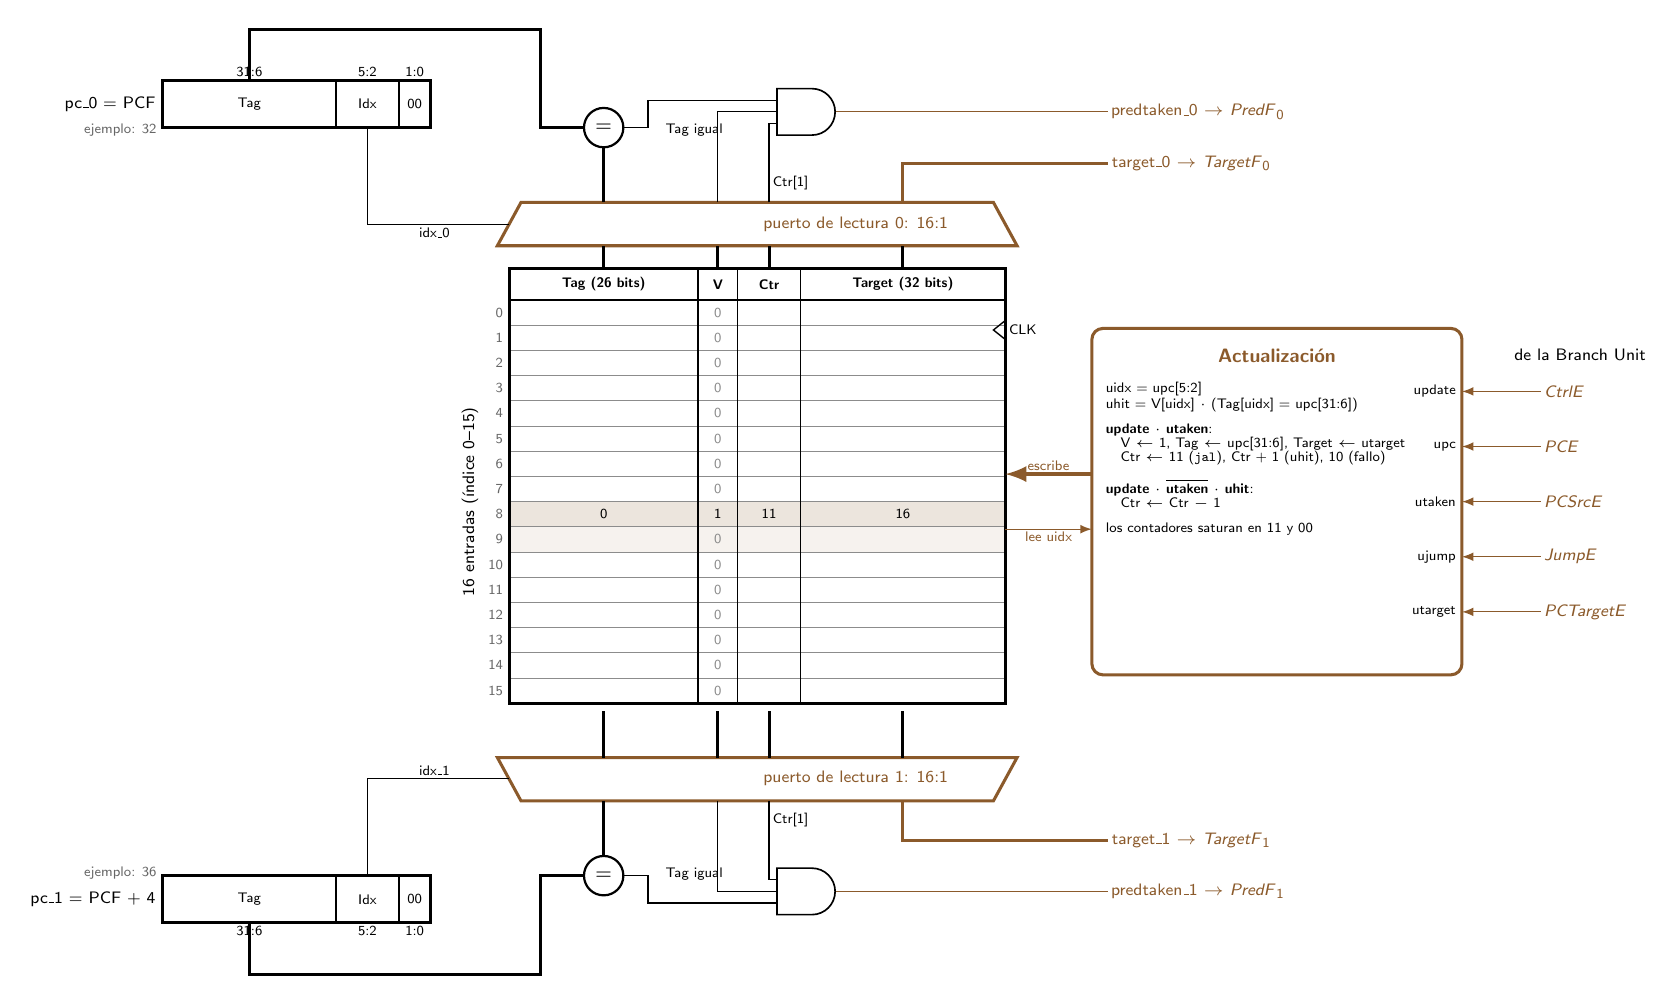
\begin{tikzpicture}[x=1cm,y=1cm, circuit logic US, small circuit symbols,
  every circuit symbol/.style={line width=0.6pt, fill=white}]
\newcommand{\Y}[1]{\fpeval{\s*(#1)}}
% columns: Tag 0-2.4, V 2.4-2.9, Ctr 2.9-3.7, Target 3.7-6.3 ; 16 rows of 0.32 (y = 2.56 .. -2.56)
\def\rh{0.32}
\fill[opt!16] (0,{2.56-8*\rh}) rectangle (6.3,{2.56-9*\rh});   % row 8 (pc_0 = 32)
\fill[opt!8]  (0,{2.56-9*\rh}) rectangle (6.3,{2.56-10*\rh});  % row 9 (pc_1 = 36)
\foreach \i in {1,...,15} \draw[line width=0.3pt, black!45] (0,{2.56-\i*\rh}) -- (6.3,{2.56-\i*\rh});
\foreach \x in {2.4,2.9,3.7} \draw[line width=0.5pt] (\x,-2.56) -- (\x,2.96);
\draw[line width=1.1pt] (0,-2.56) rectangle (6.3,2.96);
\draw[line width=0.5pt] (0,2.56) -- (6.3,2.56);
\foreach \x/\t in {1.2/Tag (26 bits), 2.65/V, 3.3/Ctr, 5.0/Target (32 bits)}
  \node[bit, font=\fontsize{5.5}{5.5}\selectfont\bfseries] at (\x,2.76) {\t};
\foreach \i in {0,...,15}
  \node[bit, anchor=east, text=black!60] at (-0.05,{2.56-(\i+0.5)*\rh}) {\i};
\foreach \i in {0,...,7,10,11,12,13,14,15}
  \node[bit, text=black!45] at (2.65,{2.56-(\i+0.5)*\rh}) {0};
% example: the beq at PC 32 of pred_slot0.s (index 8, tag 0) after it was taken twice
\foreach \x/\t in {1.2/0, 2.65/1, 3.3/11, 5.0/16} \node[bit] at (\x,{2.56-8.5*\rh}) {\t};
\node[bit, text=black!45] at (2.65,{2.56-9.5*\rh}) {0};
\node[lab, anchor=south, rotate=90] at (-0.35,0) {16 entradas (índice 0--15)};
\draw[line width=0.5pt] (6.3,2.3) -- (6.15,2.18) -- (6.3,2.06);
\node[bit, anchor=west] at (6.32,2.18) {CLK};

\foreach \s/\k/\pc/\ex in {1/0/PCF/32, -1/1/{PCF + 4}/36} {
  \ifnum\k=0 \def\va{south}\def\vb{north}\else \def\va{north}\def\vb{south}\fi
  % read port k: 16:1 multiplexer over the whole entry (V, Tag, Ctr, Target)
  \draw[line width=1.1pt, opt, fill=white] (-0.15,\Y{3.25}) -- (6.45,\Y{3.25}) -- (6.15,\Y{3.8}) -- (0.15,\Y{3.8}) -- cycle;
  \node[lab, opt] at (4.4,\Y{3.52}) {puerto de lectura \k: 16:1};
  \foreach \x in {1.2,2.65,3.3,5.0} \draw[w] (\x,\Y{2.96+0.3*(1-\s)/2*(-1)}) -- (\x,\Y{3.25});
  % address fields
  \draw[line width=1.1pt] (-4.4,\Y{4.75}) rectangle (-1.0,\Y{5.35});
  \draw[line width=0.5pt] (-2.2,\Y{4.75}) -- (-2.2,\Y{5.35});
  \draw[line width=0.5pt] (-1.4,\Y{4.75}) -- (-1.4,\Y{5.35});
  \node[bit] at (-3.3,\Y{5.05}) {Tag};  \node[bit] at (-1.8,\Y{5.05}) {Idx};  \node[bit] at (-1.2,\Y{5.05}) {00};
  \node[bit, anchor=\va] at (-3.3,\Y{5.37}) {31:6};
  \node[bit, anchor=\va] at (-1.8,\Y{5.37}) {5:2};
  \node[bit, anchor=\va] at (-1.2,\Y{5.37}) {1:0};
  \node[lab, anchor=east] at (-4.45,\Y{5.05}) {pc\_\k\ = \pc};
  \node[bit, anchor=east, text=black!60] at (-4.45,\Y{4.72}) {ejemplo: \ex};
  % index -> select of the read multiplexer
  \draw[nw] (-1.8,\Y{4.75}) -- (-1.8,\Y{3.52}) -- (0.0,\Y{3.52});
  \node[bit, anchor=\vb] at (-0.95,\Y{3.5}) {idx\_\k};
  % tag comparison
  \node[draw, circle, line width=0.8pt, inner sep=0.5pt, minimum size=0.5cm, fill=white,
        font=\fontsize{7}{7}\selectfont] (cmp\k) at (1.2,\Y{4.75}) {$=$};
  \draw[w] (1.2,\Y{3.8}) -- (cmp\k);
  \draw[w] (-3.3,\Y{5.35}) -- (-3.3,\Y{6.0}) -- (0.4,\Y{6.0}) -- (0.4,\Y{4.75}) -- (cmp\k);
  % predtaken = V & (tag equal) & Ctr[1]
  \node[and gate, inputs=nnn, anchor=output] (g\k) at (4.15,\Y{4.95}) {};
  \draw[nw] (cmp\k.east) -- ++(0.3,0) |- (g\k.input \fpeval{2-\s});
  \draw[nw] (2.65,\Y{3.8}) |- (g\k.input 2);
  \draw[nw] (3.3,\Y{3.8}) |- (g\k.input \fpeval{2+\s});
  \node[bit, anchor=\vb] at (2.35,\Y{4.83}) {Tag igual};
  \node[bit, anchor=west] at (3.32,\Y{4.05}) {Ctr[1]};
  \draw[o] (g\k.output) -- (7.6,\Y{4.95}) node[lab, opt, anchor=west] {predtaken\_\k\ $\to$ \sigk{PredF}{\k}};
  \draw[w, opt] (5.0,\Y{3.8}) -- (5.0,\Y{4.3}) -- (7.6,\Y{4.3}) node[lab, opt, anchor=west] {target\_\k\ $\to$ \sigk{TargetF}{\k}};
}

% update port (Execute): writes the entry uidx at the clock edge
\draw[line width=1.1pt, opt, rounded corners=4pt, fill=white] (7.4,-2.2) rectangle (12.1,2.2);
\node[lab, opt, font=\fontsize{7}{7}\selectfont\bfseries] at (9.75,1.85) {Actualización};
\node[bit, align=left, anchor=north west] at (7.55,1.55) {%
  uidx = upc[5:2]\\[1pt]
  uhit = V[uidx] $\cdot$ (Tag[uidx] = upc[31:6])\\[4pt]
  \textbf{update $\cdot$ utaken}:\\
  \quad V $\leftarrow$ 1, Tag $\leftarrow$ upc[31:6], Target $\leftarrow$ utarget\\
  \quad Ctr $\leftarrow$ 11 (\texttt{jal}), Ctr + 1 (uhit), 10 (fallo)\\[4pt]
  \textbf{update $\cdot$ $\overline{\mbox{utaken}}$ $\cdot$ uhit}:\\
  \quad Ctr $\leftarrow$ Ctr $-$ 1\\[4pt]
  los contadores saturan en 11 y 00};
\draw[line width=1.6pt, opt, -latex] (7.4,0.35) -- (6.3,0.35) node[bit, opt, pos=0.5, above] {escribe};
\draw[o, -latex] (6.3,-0.35) -- (7.4,-0.35) node[bit, opt, pos=0.5, below] {lee uidx};
\foreach \y/\p/\sg in {1.4/update/CtrlE, 0.7/upc/PCE, 0/utaken/PCSrcE, -0.7/ujump/JumpE, -1.4/utarget/PCTargetE} {
  \draw[o, latex-] (12.1,\y) -- (13.1,\y) node[lab, opt, anchor=west] {\sig{\sg}};
  \node[bit, anchor=east] at (12.05,\y) {\p};
}
\node[lab, anchor=south] at (13.6,1.75) {de la Branch Unit};
\end{tikzpicture}
\end{document}
